\section{Introduction} \label{sec:funtamentals}
\subsection{Why to Replicate CI / CD Locally}

\begin{frame}{High level description of the problem}
\setbeamercovered{dynamic}%Makes the text appear before it presents nice!!!!
	\begin{columns}[T] % contents are top vertically aligned
		\begin{column}{5cm} % each column can also be its own environment
			\begin{itemize}
				\item<+-| alert@+> It works locally why not remotely?
				\item<+-| alert@+> It works on my computer why not on yours?
				\item<+-| alert@+> Common Wrong Assumptions:
					\begin{itemize}
						\item<+-| alert@+> Running same package(s) version
						\item<+-| alert@+> No difference on installation process
						\item<+-| alert@+> No difference between Operating Systems
					\end{itemize}
				\item<+-| alert@+> Is there a solution?
			\end{itemize}
		\end{column}
		\begin{column}{5cm} % alternative top-align that's better for graphics
			\begin{figure}
				\only<1>{%
					\centering Local Vs Remote
					
\includegraphics[width=\columnwidth, height=0.5\textheight]{./png/personThinking}
				}%
				\only<2>{%
					\centering Not replicable
					
\includegraphics[width=\columnwidth, height=0.5\textheight]{./png/worksOnLocal}
				}%
				\only<3>{%
					\centering Wrong Assumptions
					
\includegraphics[width=\columnwidth, height=0.5\textheight]{./png/presume}
				}%
				\only<4>{%
					\centering Major / Minor Version
					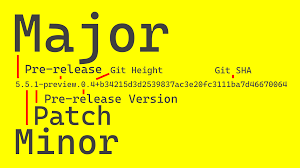
\includegraphics[width=\columnwidth, height=0.5\textheight]{./png/majorMinor}
				}%
				\only<5>{%
					\centering Is there a difference in compilers?
					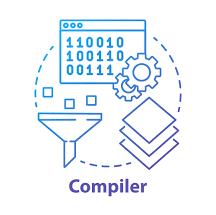
\includegraphics[width=\columnwidth, height=0.5\textheight]{./png/compiler}
				}%
				\only<6>{%
					\centering Windows vs Mac vs Linux
					
\includegraphics[width=\columnwidth, height=0.5\textheight]{./png/windowsMacLinux}
				}%
				\only<7>{%
					\centering Maybe...
					
\includegraphics[width=\columnwidth, height=0.5\textheight]{./png/letsSee}
				}%
				\caption{Problem Overview} \label{fig:largeFigure}
			\end{figure}
		\end{column}
	\end{columns}
\end{frame}
